\documentclass[12pt]{article}

\author{Jesse E.J. op den Brouw\thanks{\texttt{J.E.J.opdenBrouw@hhs.nl}}\\[2ex]The Hague University of Applied Sciences}
\title{A Minimal RISC-V processor in VHDL}
\date{\today\\[2ex]\normalsize\url{https://github.com/jesseopdenbrouw/riscv-minimal}}

\usepackage[a4paper,inner=1.0in,outer=1.2in,top=1in,bottom=1.5in,footskip=0.4in,showframe]{geometry}
\usepackage{graphicx}
\usepackage{xcolor}
\usepackage[charter]{mathdesign}
\usepackage[scale=0.92]{nimbusmono}
\usepackage{booktabs}
\usepackage{mathtools}
\usepackage{rotating}
\usepackage{register}


%% Making captions nicer...
\usepackage[font=footnotesize,format=plain,labelfont=bf,textfont=sl]{caption}
\usepackage[labelformat=simple,font=footnotesize,format=plain,labelfont=bf,textfont=sl]{subcaption}
\captionsetup[figure]{format=hang,justification=centering,singlelinecheck=off,skip=2ex}
\captionsetup[table]{format=hang,justification=centering,singlelinecheck=off,skip=2ex}
\captionsetup[subfigure]{format=hang,justification=centering,singlelinecheck=off,skip=2ex}
\captionsetup[subtable]{format=hang,justification=centering,singlelinecheck=off,skip=2ex}
%% Put parens around the subfig name (a) (b) etc. Needs labelformat simple
\renewcommand\thesubfigure{(\alph{subfigure})}
\renewcommand\thesubtable{(\alph{subtable})}

% Parskip et al.
\usepackage{parskip}
\makeatletter
\setlength{\parfillskip}{00\p@ \@plus 1fil}
\makeatother

\usepackage{listings}
\lstset{
    basicstyle = \ttfamily,
    breaklines = true,
    showspaces=false,
    prebreak = \raisebox{-0.5ex}[0ex][0ex]{\color{red}\ensuremath{\hookleftarrow}},
    postbreak = \raisebox{-0.5ex}[0ex][0ex]{\color{red}\ensuremath{\hookrightarrow}},
}

\usepackage{tikz}
\usetikzlibrary{backgrounds,shapes,arrows}

\usepackage{hyperref}
\hypersetup{colorlinks}

\begin{document}
\maketitle

\vfill
\begin{abstract}
\noindent
The RISC-V Instruction Set Architecture (ISA) is an open source instruction set for a processor. This means that anybody can create a processor that uses this instruction set. There are already processors available such as E2-core from SiFive. More freeware cores are available on several platforms (e.g. on GitHub). This documents describes a basic 32-bit RISC-V core in VHDL. The core can only execute the RV32I unprivileged instruction set. The processor incorporates a ROM, RAM and some simple I/O. It is targeted for implementation on an FPGA. It is tested on an Intel Cyclone V with a DE0-CV development board from Terasic with the use of Quartus Prime Lite 21.1 and QuestaSim Intel Starter Edition 2021.2. The GNU C-compiler for RISC-V is used for software development. Currently only simple C programs can be compiled and run. C++ is currently not supported.

\noindent
This processor is not intended as a replacement for commercial available processors. It is intended as a study object for Computer Science students. The processor executes each instruction in two clock cycles because the ROM is inferred using onboard RAM. ROM and RAM reads need an extra clock cycle. The processor has a simple, non-pipelined instruction decoder. Exceptions are currently not implemented. This will be for future development.

\noindent
This is work in progress. Things will certainly change in the future.
\end{abstract}
\vfill

\clearpage
\tableofcontents

\clearpage
\section{Introduction}
This document describes the buildup of a simple, dual/triple clock cycle, one core, RISC-V processor, completely written in VHDL. The processor is able to run a simple compiled C-program. C++ is currently not supported. The processor can handle the RV32I Base Integer Instruction Set as set forward in ``The RISC-V Instruction Set Manual Volume I: Unprivileged ISA''. The RV32M Instruction Set is currently not supported, so multiplications and divisions will be handled in software. The C-compiler will take care of that when supplied with the correct parameters. The aim is to synthesize for a minimum clock frequency of 50\,MHz.

\section{The processor in VHDL}
This RISC-V processor consists of the following building blocks:

\begin{itemize}
\item The registers contain intermediate data for calculations.
\item The ROM contains the program instructions and constant (read-only) data.
\item The RAM contains read-write data (mutable data).
\item The I/O is an interface with the outside world.
\item The ALU is responsible for almost all computations in the processor.
\item The PC is used to point to the currently executing instruction.
\item The Address Decoder and Data Router is an interface between the memory (ROM, RAM, I/O) and the ALU and registers.
\item The Instruction Decoder decodes the currently executing instruction and provides control signals to other building blocks.
\end{itemize}

A block diagram is shown in Figure~\ref{fig:blockdiagram}.

The processor uses preprogrammed onboard RAM blocks to implement the ROM. Register/register and register/immediate instructions require two clock cycles, register/memory instructions require two clock cycles for a write operations and register/memory instructions require three clock cycles for read operations.
 
\begin{sidewaysfigure}[!p]
\centering
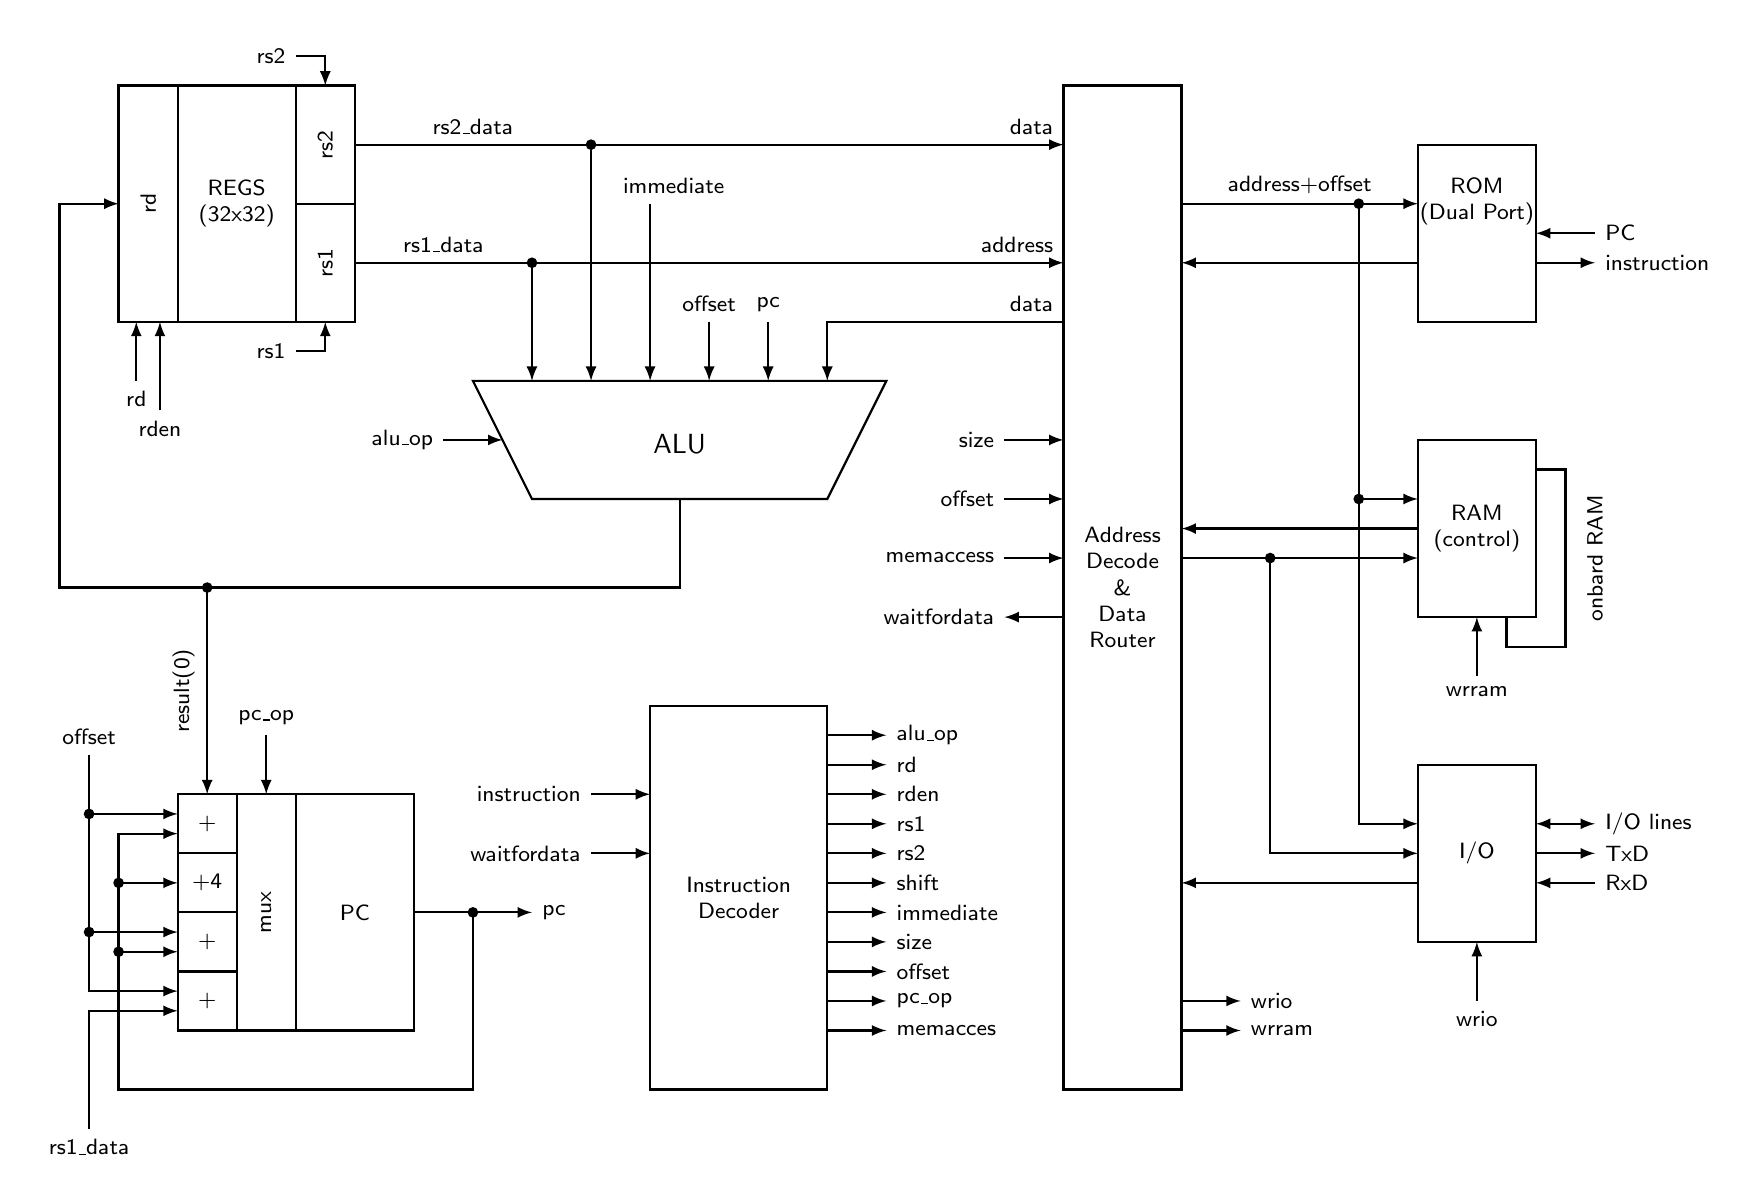
\begin{tikzpicture}[thick,font=\sffamily\footnotesize,>=latex,scale=.75,framed,background rectangle/.style={fill=none}]
% Demux and regs
\draw (0,0) rectangle (1,-4) node[midway,rotate=90] {rd};
\draw (1,0) rectangle (3,-4) node[midway,align=center] {REGS\\(32x32)};
\draw[->] (0.3,-5) node[below] {rd} -- (0.3,-4);
\draw[->] (0.7,-5.5) node[below] {rden} -- (0.7,-4);
\draw (3,0) rectangle (4,-2) node[midway,rotate=90] {rs2};
\draw[->] (3.0,0.5) node[left] {rs2} -- ++(0.5,0) -- ++(0,-0.5);
\draw (3,-2) rectangle (4,-4) node[midway,rotate=90] {rs1};
\draw[->] (3,-4.5) node[left] {rs1} -- ++(0.5,0) -- ++(0,0.5);
\draw (4,-3) -- (7,-3) node[midway,above] {rs1\_data};
\draw[->] (7,-3) -- (16,-3) node[above left] {address}; 
\draw (4,-1) -- (8,-1) node[midway,above] {rs2\_data};
\draw[->] (8,-1) -- (16,-1) node[above left] {data}; 
\draw[fill=black] (8,-1) circle (2pt);
\draw[fill=black] (7,-3) circle (2pt);

% ALU
\draw (6,-5) -- ++(7,0) node[midway,yshift=-0.8cm,font=\normalsize\sffamily] {ALU} -- ++(-1,-2) -- ++(-5,0) -- cycle;
\draw[->] (7,-3) -- (7,-5);
\draw[->] (8,-1) -- (8,-5);
\draw[->] (5.5,-6) node[left] {alu\_op} -- (6.5,-6);
\draw[->] (9.5,-7.0) -- (9.5,-8.5) -- ++(-10.5,0) -- ++(0,6.5) -- ++(1,0);
\draw[->] (11,-4.0) node[above] {pc} -- ++(0,-1);
\draw[->] (10,-4.0) node[above] {offset} -- ++(0,-1);
\draw[->] (9,-2.0) node[above,xshift=3mm] {immediate} -- ++(0,-3);

% Address decode and data route
\draw (16,-0) rectangle ++(2,-17) node[midway,align=center] {Address\\Decode\\\&\\Data\\Router};
\draw[->] (16,-4) node[above left] {data} -- ++(-4,0) -- ++(0,-1);
\draw[->] (15,-6) node[left] {size} -- ++(1,0);
\draw[->] (15,-7) node[left] {offset} -- ++(1,0);
\draw[->] (15,-8) node[left] {memaccess} -- ++(1,0);
\draw[<-] (15,-9) node[left] {waitfordata} -- ++(1,0);
\draw[->] (18,-15.5) -- ++(1,0) node[right] {wrio};
\draw[->] (18,-16.0) -- ++(1,0) node[right] {wrram};

% Instruction decoder
\draw (9,-10.5) rectangle ++(3,-6.5) node[midway,align=center] {Instruction\\Decoder};
\draw[->] (12,-11.0) -- ++(1,0) node[right] {alu\_op};
\draw[->] (12,-11.5) -- ++(1,0) node[right] {rd};
\draw[->] (12,-12.0) -- ++(1,0) node[right] {rden};
\draw[->] (12,-12.5) -- ++(1,0) node[right] {rs1};
\draw[->] (12,-13.0) -- ++(1,0) node[right] {rs2};
\draw[->] (12,-13.5) -- ++(1,0) node[right] {shift};
\draw[->] (12,-14.0) -- ++(1,0) node[right] {immediate};
\draw[->] (12,-14.5) -- ++(1,0) node[right] {size};
\draw[->] (12,-15.0) -- ++(1,0) node[right] {offset};
\draw[->] (12,-15.5) -- ++(1,0) node[right] {pc\_op};
\draw[->] (12,-16.0) -- ++(1,0) node[right] {memacces};
%\draw[->,red] (12,-16.5) -- ++(1,0) node[right] {error};
\draw[->] (8,-12) node[left] {instruction} -- ++(1,0);
\draw[->] (8,-13) node[left] {waitfordata} -- ++(1,0);
%\draw[->,red] (8,-15) node[left] {intreq} -- ++(1,0);

% ROM
\draw (22,-1) rectangle ++(2,-3) node[midway,align=center,yshift=0.4cm] {ROM\\(Dual Port)};
\draw[<-] (24,-2.5) -- ++(1,0) node[right] {PC};
\draw[->] (24,-3.0) -- ++(1,0) node[right] {instruction};
\draw[->] (18,-2) -- ++(4,0) node[midway,above] {address+offset};

% Address lines to RAM and I/O
\draw[->] (21,-2) -- ++(0,-5) -- ++(1,0);
\draw[fill=black] (21,-2) circle (2pt);
\draw[->] (21,-7) -- ++(0,-5.5) -- ++(1,0);
\draw[fill=black] (21,-7) circle (2pt);
% Data lines from ROM, RAM, I/O
\draw[->] (22,-3) -- ++(-4,0);
\draw[->] (22,-7.5) -- ++(-4,0);
\draw[->] (22,-13.5) -- ++(-4,0);
% Data lines to RAM and I/O
\draw[->] (18,-8) -- ++(1.5,0) -- ++(2.5,0);
\draw[->] (19.5,-8) -- ++(0,-5.0) -- ++(2.5,0);
\draw[fill=black] (19.5,-8) circle (2pt);

% RAM
\draw (22,-6) rectangle ++(2,-3) node[midway,align=center] {RAM\\(control)};
\draw[->] (23,-10) node[below] {wrram} -- ++(0,1);
\draw (24,-6.5) -- ++(0.5,0) -- ++(0,-3) -- ++(-1,0) -- ++(0,0.5);
\node at (25,-8) [rotate=90] {onbard RAM};

% I/O
\draw (22,-11.5) rectangle ++(2,-3) node[midway] {I/O};
\draw[->] (23,-15.5) node[below] {wrio} -- ++(0,1);
\draw[<->] (24,-12.5) -- ++(1,0) node[right] {I/O lines};
\draw[->] (24,-13) -- ++(1,0) node[right] {TxD};
\draw[<-] (24,-13.5) -- ++(1,0) node[right] {RxD};
%\draw[->] (24,-13.5) -- ++(1,0) node[right] {interrupts};

% PC
\draw (3,-12) rectangle ++(2,-4) node[midway] {PC};
\draw (2,-12) rectangle ++(1,-4) node[midway, rotate=90] {mux};
\draw[->] (5,-14) -- ++(1,0) -- ++(0,-3) -- ++ (-6,0) -- ++(0,4.333) -- ++(1,0);
\draw[->] (6,-14) -- ++(1,0) node[right] {pc};
\draw[fill=black] (6,-14) circle (2pt);
\draw[->] (0,-13.5) -- ++(1,0);
\draw[fill=black] (0,-13.5) circle (2pt);

\draw (1,-12) rectangle ++(1,-1) node[midway] {+};
\draw (1,-13) rectangle ++(1,-1) node[midway] {+4};
\draw (1,-14) rectangle ++(1,-1) node[midway] {+};
\draw (1,-15) rectangle ++(1,-1) node[midway] {+};
\draw[->] (2.5,-11) node[above] {pc\_op}-- ++(0,-1);

\draw[->] (1.5,-8.5) -- ++ (0,-3.5) node[xshift=-3mm,midway,rotate=90] {result(0)};
\draw[fill=black] (1.5,-8.5) circle (2pt);

\draw[->] (0,-14.6667) -- ++(1,0);
\draw[fill=black] (0,-14.6667) circle (2pt);

\draw[->] (-0.5,-11.333) node[above] {offset} -- ++(0,-1) -- ++(1.5,0);
\draw[->] (-0.5,-12.333) -- ++(0,-2) -- ++(1.5,0);
\draw[fill=black] (-0.5,-12.333) circle (2pt);
\draw[->] (-0.5,-14.333) -- ++(0,-1) -- ++(1.5,0);
\draw[fill=black] (-0.5,-14.333) circle (2pt);

\draw[->] (-0.5,-17.6667) node[below] {rs1\_data} -- ++(0,2) -- ++(1.5,0);
\end{tikzpicture}
\caption{The complete RISC-V MCU.}
\label{fig:blockdiagram}
\end{sidewaysfigure}



\subsection{Registers}
The processor consists of thirty-two 32-bit registers denoted by \texttt{x0} to \texttt{x31}. Internally, the registers use Big Endian format. Register \texttt{x0} (alias \texttt{zero}) is hardwired to all zeros. Writing this register has no effect. Reading this register returns all zero bits. Normally, the \texttt{x}-names are not used but may be handy when simulating the designs. Table~\ref{tab:registers} shows the names of the registers as they should be used.

A register can be written to, and two register can be selected for data and base address.

\begin{table}[!ht]
\centering
\caption{RISC-V registers and their purpose.}
\label{tab:registers}
\begin{tabular}{lllc}
Register & Name & Purpose & Saver \\
\midrule
\texttt{x0}      & \texttt{zero}   & Hard-wired zero                   & $-$ \\
\texttt{x1}      & \texttt{ra}     & Return address                    & Caller \\
\texttt{x2}      & \texttt{sp}     & Stack pointer                     & Callee \\
\texttt{x3}      & \texttt{gp}     & Global pointer                    & $-$ \\
\texttt{x4}      & \texttt{tp}     & Thread pointer                    & $-$ \\
\texttt{x5}      & \texttt{t0}     & Temporary/alternate link register & Caller \\
\texttt{x6-x7}   & \texttt{t1-t2}  & Temporaries                       & Caller \\
\texttt{x8}      & \texttt{s0/fp}  & Saved register/frame pointer      & Callee \\
\texttt{x9}      & \texttt{s1}     & Saved register                    & Callee \\
\texttt{x10-x11} & \texttt{a0-a1}  & Function arguments/return values  & Caller \\
\texttt{x12-x17} & \texttt{a2-a7}  & Function arguments                & Caller \\
\texttt{x18-x27} & \texttt{s2-s11} & Saved registers                   & Callee \\
\texttt{x28-x31} & \texttt{t3-t6}  & Temporaries                       & Caller
\end{tabular}
\end{table}

\subsection{ROM}
\label{sec:rom}
The ROM consists of bytes and is only word addressable for instructions. The ROM is byte, half word and word addressable when reading constant data. Half word and word entries are in Litte Endian format. When reading data from the ROM, halfword accesses must be on 2-byte boundaries and word accesses must be on 4-byte boundaries. This simplifies the decoding circuitry. The ROM returns undefined data if an access is not aligned. The processor instantiates the ROM in onboard RAM. Rearranging half word and word data accesses in Big Endian format is handled by the ROM decoding unit.

Note: because the ROM is instantiated using onboard RAM, each read (instruction and data) requires an extra clock cycle.

\subsection{RAM}
\label{sec:ram}
The RAM consists of bytes and is byte, halfword and word addressable. Half word and word entries are in Little Endian format. The RAM itself is made up of word (i.e. 32-bit) entries and is instantiated with onboard RAM blocks. Due to this fact, halfword accesses are only permitted on 2-byte boundaries and word accesses are only permitted on 4-byte boundaries. The RAM returns undefined data if an access is not aligned. Writes will not take place if an access is unaligned. This simplifies the decoding circuitry. For the Cyclone V a maximum of 65536 words of RAM can be instantiated. Rearranging half word and word data accesses in Big Endian format is handled by the RAM decoding unit.

Note: the Cyclone V has 3,153,920 bits of RAM available. Because of the 32-bit entries a maximum of 2,097,152 (65536 x 32) bits can be instantiated. This is equivalent to 262,144 bytes.

Writing the RAM (byte, half word of word) requires two clock cycle. Reading the RAM (byte, half word, word) requires three clock cycles because the RAM output is buffered by a register. This is automatically handled by the processor.

\subsection{I/O}
\label{sec/io}
Currently, the I/O consists of one 32-bit data input and one 32-bit data output, and a simple UART. More I/O (timers/counter, ...) will be added in the future, but most I/O requires the use of interrupts (timer overflow etc.). Note that the I/O can only be accessed as words and the addresses must be on 4-byte boundaries. If not on a 4-byte boundaries and not word size reads/writes, reads return undefined data whereas writes will not write data.

The UART can transmit and receive data at 8 bits, no parity and 1 stop bit only (8N1).

\subsection{ALU}
\label{sec:alu}
The Arithmetic and Logic Unit (ALU) handles all computations on data. It can add, subtract, do logic operations such as AND, OR en XOR, can shift data left or right, and sign extend byte and halfword data. Some operations require two registers, some only use one register. Furthermore the ALU is also used to determine if a conditional branch should be taken. Note that the RISC-V programmer's model does not incorporate status flags as some other architectures do. This requires some extra instructions when adding or subtracting double word (64-bit) data. The ALU is also used to compute the return address from unconditional function calls (JAL and JALR instructions). The data is in Big Endian format.

Note that the computation of jump target addresses is handled by the Program Counter (PC)

\subsection{PC}
\label{sec:pc}
The Program Counter contains the address of the currently executed instruction. The address is always on a 4-byte boundary although function calls and conditional jump (JAL, JALR en B$xx$ instructions) can be on non 4-byte boundaries (the C compiler will always create 4-bytes boundaries). The PC (or rather the VHDL description of the PC) handles the address calculations of jumps and branches taken.

\subsection{Instruction Decoder}
\label{sec:instructiondecoder}
The instruction decoder decodes the instruction supplied by the ROM as pointed by the PC. An instruction is 4-bytes wide and in Little Endian order. The instruction decoder provides all control signals for the ALU, the PC, the Address Decoder and the register file.

In the processor, a simple three-state FSM is used. All instructions require two clock cycles to be fetched and executed, and an extra clock cycle is needed when reading RAM or ROM. The FSM takes care of that.

The instruction decoder is non-pipelined. That simplifies the design but slows down the computational speed.

\subsection{Address Decoder and Data Router}
\label{sec:addressdecoderanddatarouter}
The Address Decoder and Data Router routes reads and writes to the ROM (only reads), RAM and the I/O. The processor uses a 32-bit linear address space for ROM, RAM and I/O. In the default setting, ROM starts at address 0x00000000 and the length is 64 kB. Unused ROM addresses return 0x0000000. The RAM starts at address 0x20000000 and length is 32 kB. The I/O starts at address 0xF0000000 and the length is 16 kB by default.

When data is read, the data is collected from the accessed memory and put on an internal bus to the ALU. The ALU can perform sign extension (byte and halfword accesses) if needed. Please note that reading data from the RAM and ROM requires an extra clock cycle. Reading data from I/O requires no extra clock cycle.

\subsection{Stack pointer}
The stack pointer is fully implemented although the ISA does not provide pushes and pops. The stack pointer is used to allocate local variables and is updated with each allocation and deallocation. As usual, the stack grows downwards (to lower addresses) on allocations and upwards (to higher addresses) on deallocations. Therefore the stack pointer is set to the highest RAM address + 1 on startup (which is 0x20008000 by default). The ISA postulates that the stack is aligned on 16-byte boundaries.

\subsection{Implemented instructions}
All RV32I Unprivileged instructions are implemented with the exception of FENCE, ECALL and EBREAK instructions. These instructions act as a no-operation (NOP). This is because exceptions are not implemented.

\section{The FPGA}
For this project, we use the Cyclone V FPGA from Intel (formerly Altera). See \url{https://www.intel.com/content/www/us/en/products/details/fpga/cyclone/v.html}.
The used Cyclone V is the 5CEFA4F23C7 which has 18480 ALMs available. It has 3080 kb of onboard RAM bits available which are used for RAM and ROM. Depending on the program and used resources, the compiled RISC-V processor uses about 2000-2500 ALMs (about 12\,\% - 15\,\%). This FPGA is mounted on a Terasic DE0-CV board, see \url{http://www.terasic.com.tw/cgi-bin/page/archive.pl?Language=English&No=921}. For downloading the program file, the onboard USB-Blaster is used.

It is possible to add the Quartus' Signal Tap (embedded) Logic Analyzer. Follow the instructions on \url{https://people.ece.cornell.edu/land/courses/ece5760/Quartus/Signal_tap.html}.

\section{Simulation}
The designs can be simulated fully, using QuestaSim Intel Starter or ModelSim Intel Starter. You need a (free) license for QuestaSim. During simulation, all essential signals can be viewed, as is the RAM. The RAM is viewed as 32-bit entries, so we need to do some manual calculations to correctly find byte, halfword and word accesses. Simulation can be started from Quartus.

\section{Cloning the RISC-V project}
\label{sec:cloning}
Now we have to clone the RISC-V project. It incorporates the full Quartus Prime Lite project with the processor written in VHDL. It also incorporates some simple C program examples and a taylor-made program to convert a RISC-V executable to a VHDL table suitable for the ROM. Create a working directory (and change to that directory) and issue the command:

\begin{lstlisting}[language=]
git clone https:/github.com/jesseopdenbrouw/riscv-minimal
\end{lstlisting}

In the created directory, you will see the following directories:

\texttt{CODE} -- Sample software programs, linker script and startup files\\
\texttt{DOCS} -- Documentation\\
\texttt{HARDWARE} -- the VHDL description \\
\texttt{OLD} -- yes, really old files for backup

Change directory to \texttt{CODE}. Make sure the RISC-V C compiler is available (see Section~\ref{sec:ccompiler}) and is in your path environment variable. Now enter the command \texttt{make}. It will compile all programs and the taylor-made conversion program. To clean up the programs, issue the command \texttt{make clean}.

Next, start your Quartus Prime Lite software and open the project in the \texttt{HARDWARE} directory. Now start a build by clicking on the play-symbol. It should compile a standard setting (this takes a long time). When finished, you can download the FPGA contents to the DE0-CV board.

To test one of the programs, change directory to one of the directories and copy the file with \texttt{.vhd} extension to the directory containing the VHDL description under the name \texttt{processor\_common\_rom.vhd}.
Now start Quartus and start the compilation. After a successful compilation, you can program the Cyclone V on a DE0-CV board.

\section{Setting up the GNU C compiler for \textit{this} RISC-V}
\label{sec:ccompiler}
The processor can run simple compiled C-programs that are compiled using the GNU C-compiler for RISC-V. Besides that, a separate linker script is needed to setup the compiled code. Building the C compiler (from Linux) is straightforward:

\begin{enumerate}
\item You need a current GNU C-compiler installed or your Linux box.
\item You need the texinfo package. On Ubuntu et al.\@ issue
\begin{lstlisting}[language=]
apt install texinfo
\end{lstlisting}
\item In your home directory, enter the command
\begin{lstlisting}[language=]
git clone --recursive https://github.com/riscv/riscv-gnu-toolchain
\end{lstlisting}
\item Wait for the cloning to end (takes a long time, about 30 minutes on a Zbook G5 2020 with a 10 MB/s internet connection)
\item Change to the directory with
\begin{lstlisting}[language=]
cd riscv-gnu-toolchain
\end{lstlisting}
\item Make the \texttt{build} directory with:
\begin{lstlisting}[language=]
mkdir build; cd build
\end{lstlisting}
\item Check the current configuration with
\begin{lstlisting}[language=]
../configure --help | grep abi
\end{lstlisting}
      It should say:
\begin{lstlisting}[language=]
--with-abi=lp64d    Sets the base RISC-V ABI, defaults to lp64d
\end{lstlisting}
The toolchain is currently configured for 64-bit RISC-V. That is not what we want.
\item Enter:
\begin{lstlisting}[language=]
../configure --prefix=/opt/riscv32 --with-arch=rv32i --with-abi=ilp32
\end{lstlisting}
This will set the architecture to RV32I and the ABI to ipl32. This means that integers, long integers and pointers use 32-bit entries. The destination directory is \lstinline|/opt/riscv32|
\item Now enter the make command as root: \lstinline|make|\\
MAKE SURE TO ENTER THIS COMMAND AS root, because the toolchain is put in \lstinline|/opt/riscv32|. This takes a long time (about 45 minutes on a Zbook G5). At some points the compilation seems to hang, but it is just compiling complicated C-files. By the way, you will see a lot of warnings.
\item Now that the toolchain is setup, we have to put the path into the \lstinline|$PATH| environment variable so enter
\begin{lstlisting}[language=]
export PATH=/opt/riscv32/bin:$PATH
\end{lstlisting}
\item Check if the compiler is available:
\begin{lstlisting}[language=]
riscv32-unknown-elf-gcc -v
\end{lstlisting}
It should say something like:
\begin{lstlisting}[language=]
Using built-in specs.
COLLECT_GCC=riscv32-unknown-elf-gcc
COLLECT_LTO_WRAPPER=/opt/riscv32/libexec/gcc/riscv32-unknown-elf/11.1.0/lto-wrapper
Target: riscv32-unknown-elf
Configured with: /mnt/d/PROJECTS/RISCVDEV/riscv-gnu-toolchain/build/../riscv-gcc/configure --target=riscv32-unknown-elf --prefix=/opt/riscv32 --disable-shared --disable-threads --enable-languages=c,c++ --with-system-zlib --enable-tls --with-newlib --with-sysroot=/opt/riscv32/riscv32-unknown-elf --with-native-system-header-dir=/include --disable-libmudflap --disable-libssp --disable-libquadmath --disable-libgomp --disable-nls --disable-tm-clone-registry --src=../../riscv-gcc --disable-multilib --with-abi=ilp32 --with-arch=rv32i --with-tune=rocket 'CFLAGS_FOR_TARGET=-Os   -mcmodel=medlow' 'CXXFLAGS_FOR_TARGET=-Os   -mcmodel=medlow'
Thread model: single
Supported LTO compression algorithms: zlib
gcc version 11.1.0 (GCC) 
\end{lstlisting}
\end{enumerate}

\subsection{Register subset}
It is possible to compile the toolchain to only use register \texttt{x0} to \texttt{x15}. This is called the RISC-V E extension. As a positive side effect, the register file can be cut down from 32 registers to 16 registers. This will lower the cell count and possible speed up the device. A negative side effect is that the pressure on register allocation is higher, possibly increasing instruction count when saving registers on the stack.

To configure the GNU C compiler for the E extension issue the command:

\begin{lstlisting}[language=]
../configure --prefix=/opt/riscv32 --with-arch=rv32e --with-abi=ilp32e
\end{lstlisting}

and build the compiler.

Now compile a C program with:

\begin{lstlisting}[language=]
riscv32-unknown-elf-gcc -O0 -g -o flash flash.c -Wall -T ../ldfiles/riscv.ld -march=rv32e -mabi=ilp32e -nostartfiles --specs=nano.specs ../crt/startup.c
\end{lstlisting}

Make sure to use \texttt{-march=rv32e} and \texttt{-mabi=ilp32e}.


\section{Compiling a C program by hand}
Note: only very simple C programs can be compiled for the processor at this time. We tested some simple looping (with \texttt{for}) and reading/writing the I/O. We did test the use of the C library (malloc et al, floats and double calculation, some trigonometry  functions from the mathematical library), but more tests are needed.

Compiling a program requires the following steps:

\begin{itemize}
\item In the program directory \lstinline|CODE|, create a new directory and change to that directory.
\item Create a C program file, we assume \lstinline|flash.c|.
\item Now issue the command:
\begin{lstlisting}[language=]
riscv32-unknown-elf-gcc -O2 -g -o flash flash.c -Wall -T ../ldfiles/riscv.ld -march=rv32i -nostartfiles --specs=nano.specs ../crt/startup.c
\end{lstlisting}
We supply our own linker file (\lstinline|-T ../ldfiles/riscv.ld|) and we supply our own startup file (\lstinline|../crt/startup.c|). Make sure to use \lstinline|-nostartupfiles| otherwise the default startup file will be linked and errors will report. There a three startup files:
\begin{itemize}
\item \texttt{empty.S} -- Empty startup file only providing the entry symbol. Can be used with assembler programs.
\item \texttt{minimal.S} -- Provides the entry symbol, loads the global pointer and stack pointer and calls \texttt{main}. On return of \texttt{main}, it waits in an endless loop. Can be used with minimalistic C programs.
\item \texttt{startup.c} -- Full support for C programs. Can be used with \texttt{malloc} et al.
\end{itemize}
\item Next issue the command:
\begin{lstlisting}[language=]
riscv32-unknown-elf-objcopy -O srec flash flash.srec
\end{lstlisting}
This will create an S-record file in Motorola hex-format.
\item Next issue the command:
\begin{lstlisting}[language=]
../bin/srec2vhdl -wf flash.srec flash.vhd
\end{lstlisting}
This will create a VHDL file with the ROM encoded as 32-bit Little Endian quantities. Note: the taylor-made \texttt{srec2vhdl} has to be compiled before. See Section~\ref{sec:cloning}.
\item Next issue the command:
\begin{lstlisting}[language=]
cp flash.vhd ../../HARDWARE/riscv/processor_common_rom.vhd
\end{lstlisting}
This will copy the VHDL file to the RISC-V processor ROM file.
\item Now start the compilation of the VHDL code in Quartus Prime Lite and program the compiled file. This file has the extension \lstinline|.sof|. See Figures~\ref{quartus1} to~\ref{programmer}.

\begin{figure}[!ht]
\centering
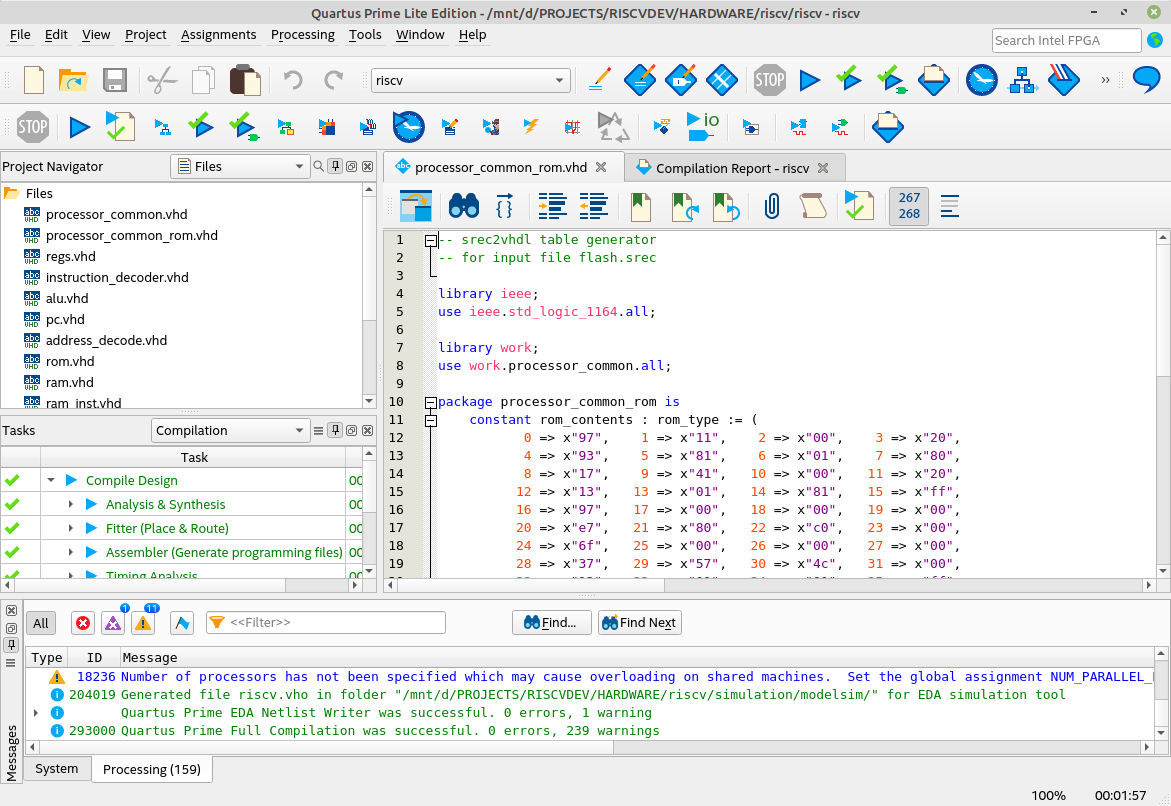
\includegraphics[width=0.85\textwidth]{quartus1}
\caption{Image of the Quartus project (1).}
\label{quartus1}
\end{figure}

\begin{figure}[!ht]
\centering
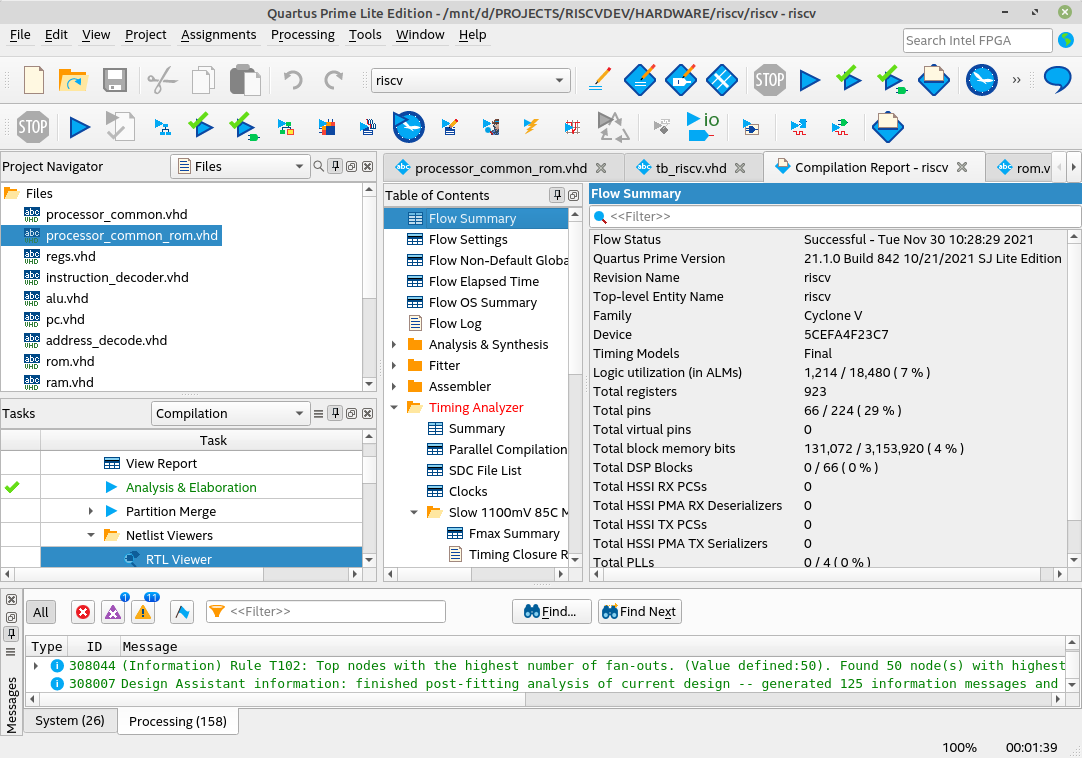
\includegraphics[width=0.85\textwidth]{quartus2}
\caption{Image of the Quartus project (2).}
\label{quartus2}
\end{figure}

\begin{figure}[!ht]
\centering
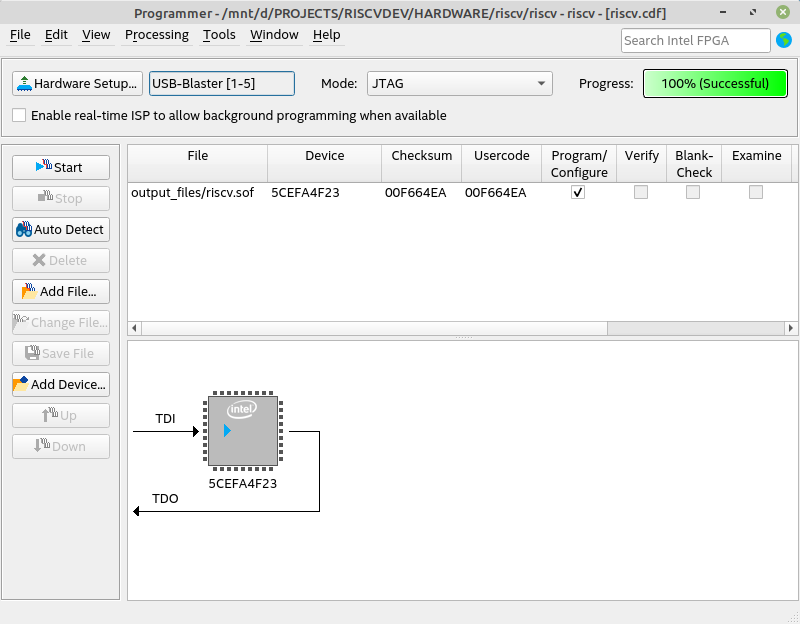
\includegraphics[width=0.85\textwidth]{programmer}
\caption{Image of the programmer.}
\label{programmer}
\end{figure}

\end{itemize}

\section{VHDL files}
Both descriptions are composed of the following files:

\begin{itemize}
\item \lstinline|processor_common.vhd| -- Common types and constants.
\item \lstinline|processor_common_rom.vhd| -- Description of the ROM contents.
\item \lstinline|address_decode.vhd| -- The address decoder and data router to the memory (ROM, RAM, I/O).
\item \lstinline|alu.vhd| -- Description of the ALU.
\item \lstinline|pc.vhd| -- Description of the Program Counter.
\item \lstinline|instruction_decoder.vhd| -- The instruction decoder.
\item \lstinline|regs.vhd| -- Description of the register file.
\item \lstinline|rom.vhd| -- Description of the ROM interface between the core and the ROM contents.
\item \lstinline|rom_inst.vhd| -- Description of the ROM contents. The ROM contents will be placed in onboard, initialized RAM blocks. The file \lstinline|rom.vhd| is then a frontend between the address decoder and data router and the onboard ROM.
\item \lstinline|ram.vhd| -- Description of the RAM interface between the address decoder and data router and the onboard RAM.
\item \lstinline|ram_inst.vhd| -- Description of the onboard RAM. Quartus detects this and creates the RAM in onboard RAM blocks.
\item \lstinline|io.vhd| -- Description of the I/O. It contains a 32-bit input register, a 32-bit output register and a simple 8-bit UART.
\item \lstinline|riscv.vhd| -- Top-level description of the processor.
\item \lstinline|riscv.sdc| -- Constraints file. Sets the target clock frequency.
\item \lstinline|tb_riscv.vhd| -- VHDL testbench to simulate the design.
\item \lstinline|tb_riscv.do| -- QuestaSim/Modelsim command script.
\end{itemize}

\section{srec2vhdl}
This is a homebrew utility to convert a Motorola S-record file into a VHDL file suitable for inclusion of the processor. The program is called with:

\begin{lstlisting}[language=c]
srec2vhdl [-fbwhqv] [-i <arg>] inputfile [outputfile]
\end{lstlisting}

\texttt{inputfile} is the S-record file, created by the \texttt{objdump} program. \texttt{outputfile} is the VHDL outputfile. When omitted, \texttt{stdout} is used. There are a number of options:

\begin{itemize}
\item \texttt{-f} makes a full output that directly can be used. If not used, only the ROM table contents itself is produced.
\item \texttt{-w} ROM contents is in words (32 bits).
\item \texttt{-h} ROM contents is in halfwords (16 bits).
\item \texttt{-b} ROM contents is in bytes (8 bits).
\item \texttt{-v} Verbose output
\item \texttt{-q} Quiet output, only error messages are displayed.
\item \texttt{-i <arg>} indents each line with \texttt{<arg>} spaces.
\end{itemize}

\section{Software programs}
In de \texttt{CODE} directory, there are a number of software programs available:

\begin{itemize}
\item \texttt{ldfiles} -- contains the linker scripts. There a two scripts:
\begin{itemize}
%\item \texttt{riscv.ld} -- default linker script with 16 kB for ROM, RAM and I/O
\item \texttt{riscv.ld} -- default linker script: ROM = 64 kB, RAM = 32 kB, I/O = 64 kB.
\end{itemize}
\item \texttt{crt} -- contains the startup files.
\item \texttt{bin} -- contains the binary of \texttt{srec2vhdl}.
\item \texttt{add64} -- simple 64-bit addition.
\item \texttt{assembler} -- a simple assembler program.
\item \texttt{ctest} -- scratch C-program test.
\item \texttt{double} -- some floating point double computations (seems to work).
\item \texttt{flash} -- flash the DE0-CV board leds (works on the board)
\item \texttt{float} -- some floating point float computations (seems to work).
\item \texttt{global} -- test for globals and local statics with initialization (seems to works).
\item \texttt{malloc} -- example to test \texttt{malloc} and friends (seems to work).
\item \texttt{mult} -- integer multiplication (works).
\item \texttt{shift} -- shifts (works)
\item \texttt{sprintf} -- prints integers, floats/doubles to a string. This is a big binary (seems to work).
\item \texttt{string} -- some string functions (seems to work).
\item \texttt{syscalls} -- implementing stubs for common system calls (seems to work). Note: \texttt{sbrk} works for \texttt{malloc}, needs more testing.
\item \texttt{testio} -- simple program that copies the input (switches) to the output (leds) (works on the board).
\item \texttt{trig} -- some float trigonometry functions (seems to work).
\item \texttt{ioadd} -- adds the lower 5 switches to the upper 5 switches and displays the result on the leds. Tests addition, shifting and I/O (works on the board).
\end{itemize} 

Note: we use a lot of the \texttt{volatile} keyword to emit the variables to RAM for easy inspection.

Note that the floating point programs loads (huge) functions from the C library and possibly creates a binary that is to large to fit in the ROM. In that case, the linker will issue an error and does not build the binary. You have to update the data sizes in the VHDL description and update the linker script with suitable data sizes.

\section{Address ranges and memory sizes}
By default, the ROM starts at address 0x00000000 and and has a size of 64 kB (16 k words). The Program Counter starts at address 0x00000000. The RAM starts at address 0x20000000 and has a size of 32 kB (8 k words). The stack pointer is set to one address above the last RAM byte, by default at 0x20008000. The I/O starts at address 0xF0000000 and has a size of 16 kB (4 k words).

The ROM, RAM and I/O may be moved to another start location. The Program Counter is started at the correct address. The placement of the ROM is in 256 MB intervals, which are the 4 most significant bits of a 32-bit address. The same holds for the RAM and the I/O. To move the ROM, open the VHDL file \lstinline|processor_common.vhd| and go down to the end of the file. There you will see the following lines:

\begin{lstlisting}[language=VHDL]
-- The highest nibble (4 bits) of the ROM, RAM and I/O
-- This will set the memories at 256 MB intervals
constant rom_high_nibble : std_logic_vector(3 downto 0) := x"0";
constant ram_high_nibble : std_logic_vector(3 downto 0) := x"2";
constant io_high_nibble : std_logic_vector(3 downto 0) := x"F";
\end{lstlisting}

Change the start locations of the memories by changing the constants. Make sure the memories do not overlap. To change the sizes of the memory, look for the lines as shown below:

\begin{lstlisting}[language=VHDL]
-- The ROM
-- NOTE: the ROM is word (32 bits) size.
-- NOTE: data is in Little Endian format (as by the toolchain)
--       for halfword and word entities
--       Set rom_size_bits as if it were bytes
-- NOTE: rom_size_bits must be <= 16
constant rom_size_bits : integer := 16;
constant rom_size : integer := 2**(rom_size_bits-2);
type rom_type is array(0 to rom_size-1) of std_logic_vector(31 downto 0);
-- The contents of the ROM is loaded by processor_common_rom.vhd

-- The RAM
-- NOTE: the RAM is 4x byte (8 bits) size, supporting
--       32-bit Big Endian storage,
--       so we have to recode to support Little Endian.
--       Set ram_size_bits as if it were bytes
-- NOTE: ram_size_bits must be <= 16
constant ram_size_bits : integer := 15;
constant ram_size : integer := 2**(ram_size_bits-2);
-- The type of the RAM block, there are 4 blocks instantiated
type ram_type is array (0 to ram_size-1) of std_logic_vector(7 downto 0);
                    
-- The I/O
-- NOTE: the I/O is word (32 bits) size, Big Endian
--       there is no need to recode the data
--       The I/O can only handle word size access
--       Set io_size_bits as if it were bytes
constant io_size_bits : integer := 6;
constant io_size : integer := 2**(io_size_bits-2);
type io_type is array (0 to io_size-1) of data_type;
\end{lstlisting}

In this setting, the ROM is 64 kB long and the RAM is 32 kB long. Please note that both ROM and RAM bits may not exceed 3,153,920 bits. For increased ROM and RAM size, typical values may be 128 kB ROM and 64 kB RAM.

%Next, open de linker script in \lstinline|<...>/ldfiles/riscv.ld|.
%
%Find the lines as showed below:
%
%\begin{lstlisting}[language=]
%MEMORY
%{
%   ROM (rx)   : ORIGIN = 0x00000000, LENGTH = 16K
%   RAM (rwx)  : ORIGIN = 0x20000000, LENGTH = 16K
%   IO (rw)    : ORIGIN = 0xf0000000, LENGTH = 16K
%}
%\end{lstlisting}
%
%Change the start addresses at the top op the file and changes the sizes if needed.
%Then recompile your programs.

\section{Future plans}
Some future plans:

\begin{itemize}
\item Implement exceptions and interrupts in general. This will bring the possibility to add more I/O, such as timers. This needs implementation of the ``Zicsr'' standard.
\item Implement the M standard: multiplier and divider. Multiplication can be achieved with the onboard multipliers but division has to be handled with a multi-cycle FSM.
\item Implement more General Purpose I/O (pins), with data direction registers. On the Cyclone V this is an issue, since the tri-state buffers must be in the top level of the design. This makes it hard to implement this processor as part of greater design.
\item Test more functions of the standard and mathematical libraries. Now only a few functions are tested.
\item Implement a simple 2-stage pipeline. The ROM is created with onboard RAM blocks and after setting an address, a read requires an clock cycle to fetch the selected ROM contents (for both instruction and data).
\end{itemize}

\section{Author's note}
I managed to create this basic RISC-V processor within one week, including compiling the GNU C compiler and the created C program examples. Of course, this is not the fastest core available, but it gives a good example on designing a RISC-V processor yourself. Next in line is to make the standard C library work. In the mean time, files will change, so be sure to grab the latest GitHub repository clone.

\appendix
\section{I/O registers}

This is a list of currently supported I/O addresses. 
The default start address is 0xF0000000. The offset is given in bytes. Note that the I/O can only be accesses on 4-byte boundaries and on word size accesses.

%\begin{register}{H}{PIN$x$}{0x00$+3x$}%
\begin{register}{H}{Port input register PIN$x$}{0x00}%
\label{pinx}%
\regfield{PIN$x$}{32}{0}{{0}}% READ_ONLY
\reglabel{Reset}\regnewline%
\end{register}

%\begin{register}{H}{PIN$x$}{0x01$+3x$}%
\begin{register}{H}{Port output register POUT$x$}{0x04}%
\label{poutx}%
\regfield{POUT$x$}{32}{0}{{0}}
\reglabel{Reset}\regnewline%
\end{register}

\begin{register}{H}{Usart data register USART\_DATA}{0x20}
\label{usartdata}
\regfield{Reserved}{24}{8}{{0}}%
\regfield{Data}{8}{0}{{0}}%
\reglabel{Reset}\regnewline%
\end{register}
\begin{regdesc}[0.6\textwidth]\begin{reglist}[000000000]
\itemsep-1.5ex
\item[Write] The data is written to an internal buffer and transmitted.
\item[Read] The last received data is read.
\end{reglist}\end{regdesc}

\begin{register}{H}{USART baud rate register USART\_BAUD}{0x24}
\label{usartbaud}
\regfield{Rerserved}{16}{16}{{0}}%
\regfield{Prescaler}{16}{0}{{0}}%
\reglabel{Reset}\regnewline%
\end{register}
\begin{regdesc}[0.6\textwidth]\begin{reglist}[000000000]
\itemsep-1.5ex
\item[Prescaler] Baud rate = $\dfrac{f_{system}}{\textrm{prescaler}+1}$
\end{reglist}\end{regdesc}

\begin{register}{H}{USART control register USART\_CTRL}{0x28}
\label{usartctrl}
\regfield{Reserved}{32}{0}{{0}}%
%\regfield{Rerserved}{16}{16}{{0}}
%\regfield{Prescaler}{16}{0}{{0}}
\reglabel{Reset}\regnewline%
\end{register}
\begin{regdesc}[0.6\textwidth]\begin{reglist}[00000]
\itemsep-1.5ex
\item [note:] currently no bits are assigned to the Control Register.
%\item[Stop Bits] Meaning
%\item[0] 1 Stop bit
%\item[1] 2 Stop bits
%\item
%\item[Parity] Meaning
%\item[00] No parity
%\item[01] Reserved
%\item[10] Even parity
%\item[11] Odd parity
%\item
%\item[Data bits]
%\item[0] 8 bits
%\item[9] 9 bits
\end{reglist}\end{regdesc}


\begin{register}{H}{USART status register USART\_STAT}{0x2c}
\label{usartstat}
\regfield{reserved}{27}{5}{{0}}%
\regfield{TC}{1}{4}{{0}}%
\regfield{Reserved}{1}{3}{{0}}%
\regfield{RC}{1}{2}{{0}}%
\regfield{RF}{1}{1}{{0}}%
\regfield{FE}{1}{0}{{0}}%
\reglabel{Reset}\regnewline%
\end{register}
\begin{regdesc}[0.8\textwidth]\begin{reglist}[0000]
\itemsep-1.5ex
\item[TC] Transmit completed. Set to 1 when a character is transmitted. Automatically cleared when writing new character or when writing 0 in the USART\_STAT bit.
\item[RC] Receive completed. Set to 1 when a character is received. Automatically cleared when receiving new character or when writing 0 in the USART\_STAT bit.
\item[RF] Receive failed. Set to 1 when failed receiving (invalid start bit). Automatically cleared when receiving new character or when writing 0 in the USART\_STAT bit.
\item [FE] Frame error. Set to 1 when a low is detected at the position of the stop bit. Automatically cleared when receiving a new character or writing a 0 in the USART\_STAT bit.
\end{reglist}\end{regdesc}

%\lstinputlisting[language=VHDL,basicstyle=\small\ttfamily]{../HARDWARE/riscv/processor_common.vhd}

%\lstinputlisting[language=VHDL,basicstyle=\small\ttfamily]{../HARDWARE/riscv/processor_common_rom.vhd}

\end{document}